\label{chap:moses}

\todo{This whole chapter is VERY dense and VERY technical. I will have to rewrite it to something more readable..... MAYBE... DAMN THERE IS NO  TIME FOR ANYTHING}

Altough our initial plan was to show translation memory only to the translator, we found out that we can also use the corpus to train a model for statistical translation. However, we also found out that despite getting quite good results from the translation, the durations for getting the translations were too long, compared to translation memory.

In this chapter, we will describe, how we trained the models, what were our results and how we managed to get the time down. The final model is a part of our project; the script to produce the model from the aligned data is not included, since it would require changes to EMS source code, which are untested at the moment and beyond the scope of this project.

Since we focus mainly on English to Czech translation, we modeled, trained and tested only for this way of translation. Training for opposite way of translation would be possible, too, but all the necessary resources would double, while the benefit would be only small and for a small number of people.

This chapter requires some knowledge of phrase-based translation models and Moses in general. If you are not familiar, the short version of this chapter is that we are getting -- on subtitles -- better results with our machine translation than Google Translate, we are getting it fast, and we were able to fit it on a rather small virtual machine.


\section{Initial set-up}
\subsection{Initial settings}
For training machine translation, we use the corpus, aligned by techniques described in section XXX. Since we want to be more exact in this case, we used more strict alignment, with 0.6\,s tolerance.

We don't need all the metadata about movie files for this task, so we added all the data together. We took away 15,000 sentences for MERT tuning (which showed up as too much) and 5,000 sentences for testing. The rest is training data.

Because of the way we took the testing sentences, they are all from different movies than the training data, except for at most one movie, that can have different sentences both in tuning and testing.

We run the standard EMS\footnote{EMS is Experiment Management System, system for managing Moses experiments, \url{http://www.statmt.org/moses/?n=FactoredTraining.EMS}} scenario on our data, which includes testing and counting BLEU score\footnote{BLEU is an automatic measurement of success of a translation}. Altough EMS counts both case-sensitive and case-insensitive BLEU, we chose the case insensitive one.

 We chose EMS instead of UFAL's own \texttt{eman}, simply for better documentation of the former and the inclusion of EMS in standard Moses installation.

Initially, for language model, we chose IRSTLM\footnote{\url{http://hlt.fbk.eu/en/irstlm}} language model. For the translation model training, we used standard GIZA++.

We also measured the time for running the test translation.\footnote{This was achhieved by adding time tracking code to EMS source code; this code was submitted to Moses and actually ``survived'' in the main git repository for a few weeks, but was ultimately deleted, because it broke some edge cases.} Time was measured on a machine with Intel Core2 Quad CPU Q9550, with 4 cores with 2.83GHz, and 4GB of memory.

For reference on quality, we also translated the test set by Google Translate.

\begin{figure}[h]
\begin{center}
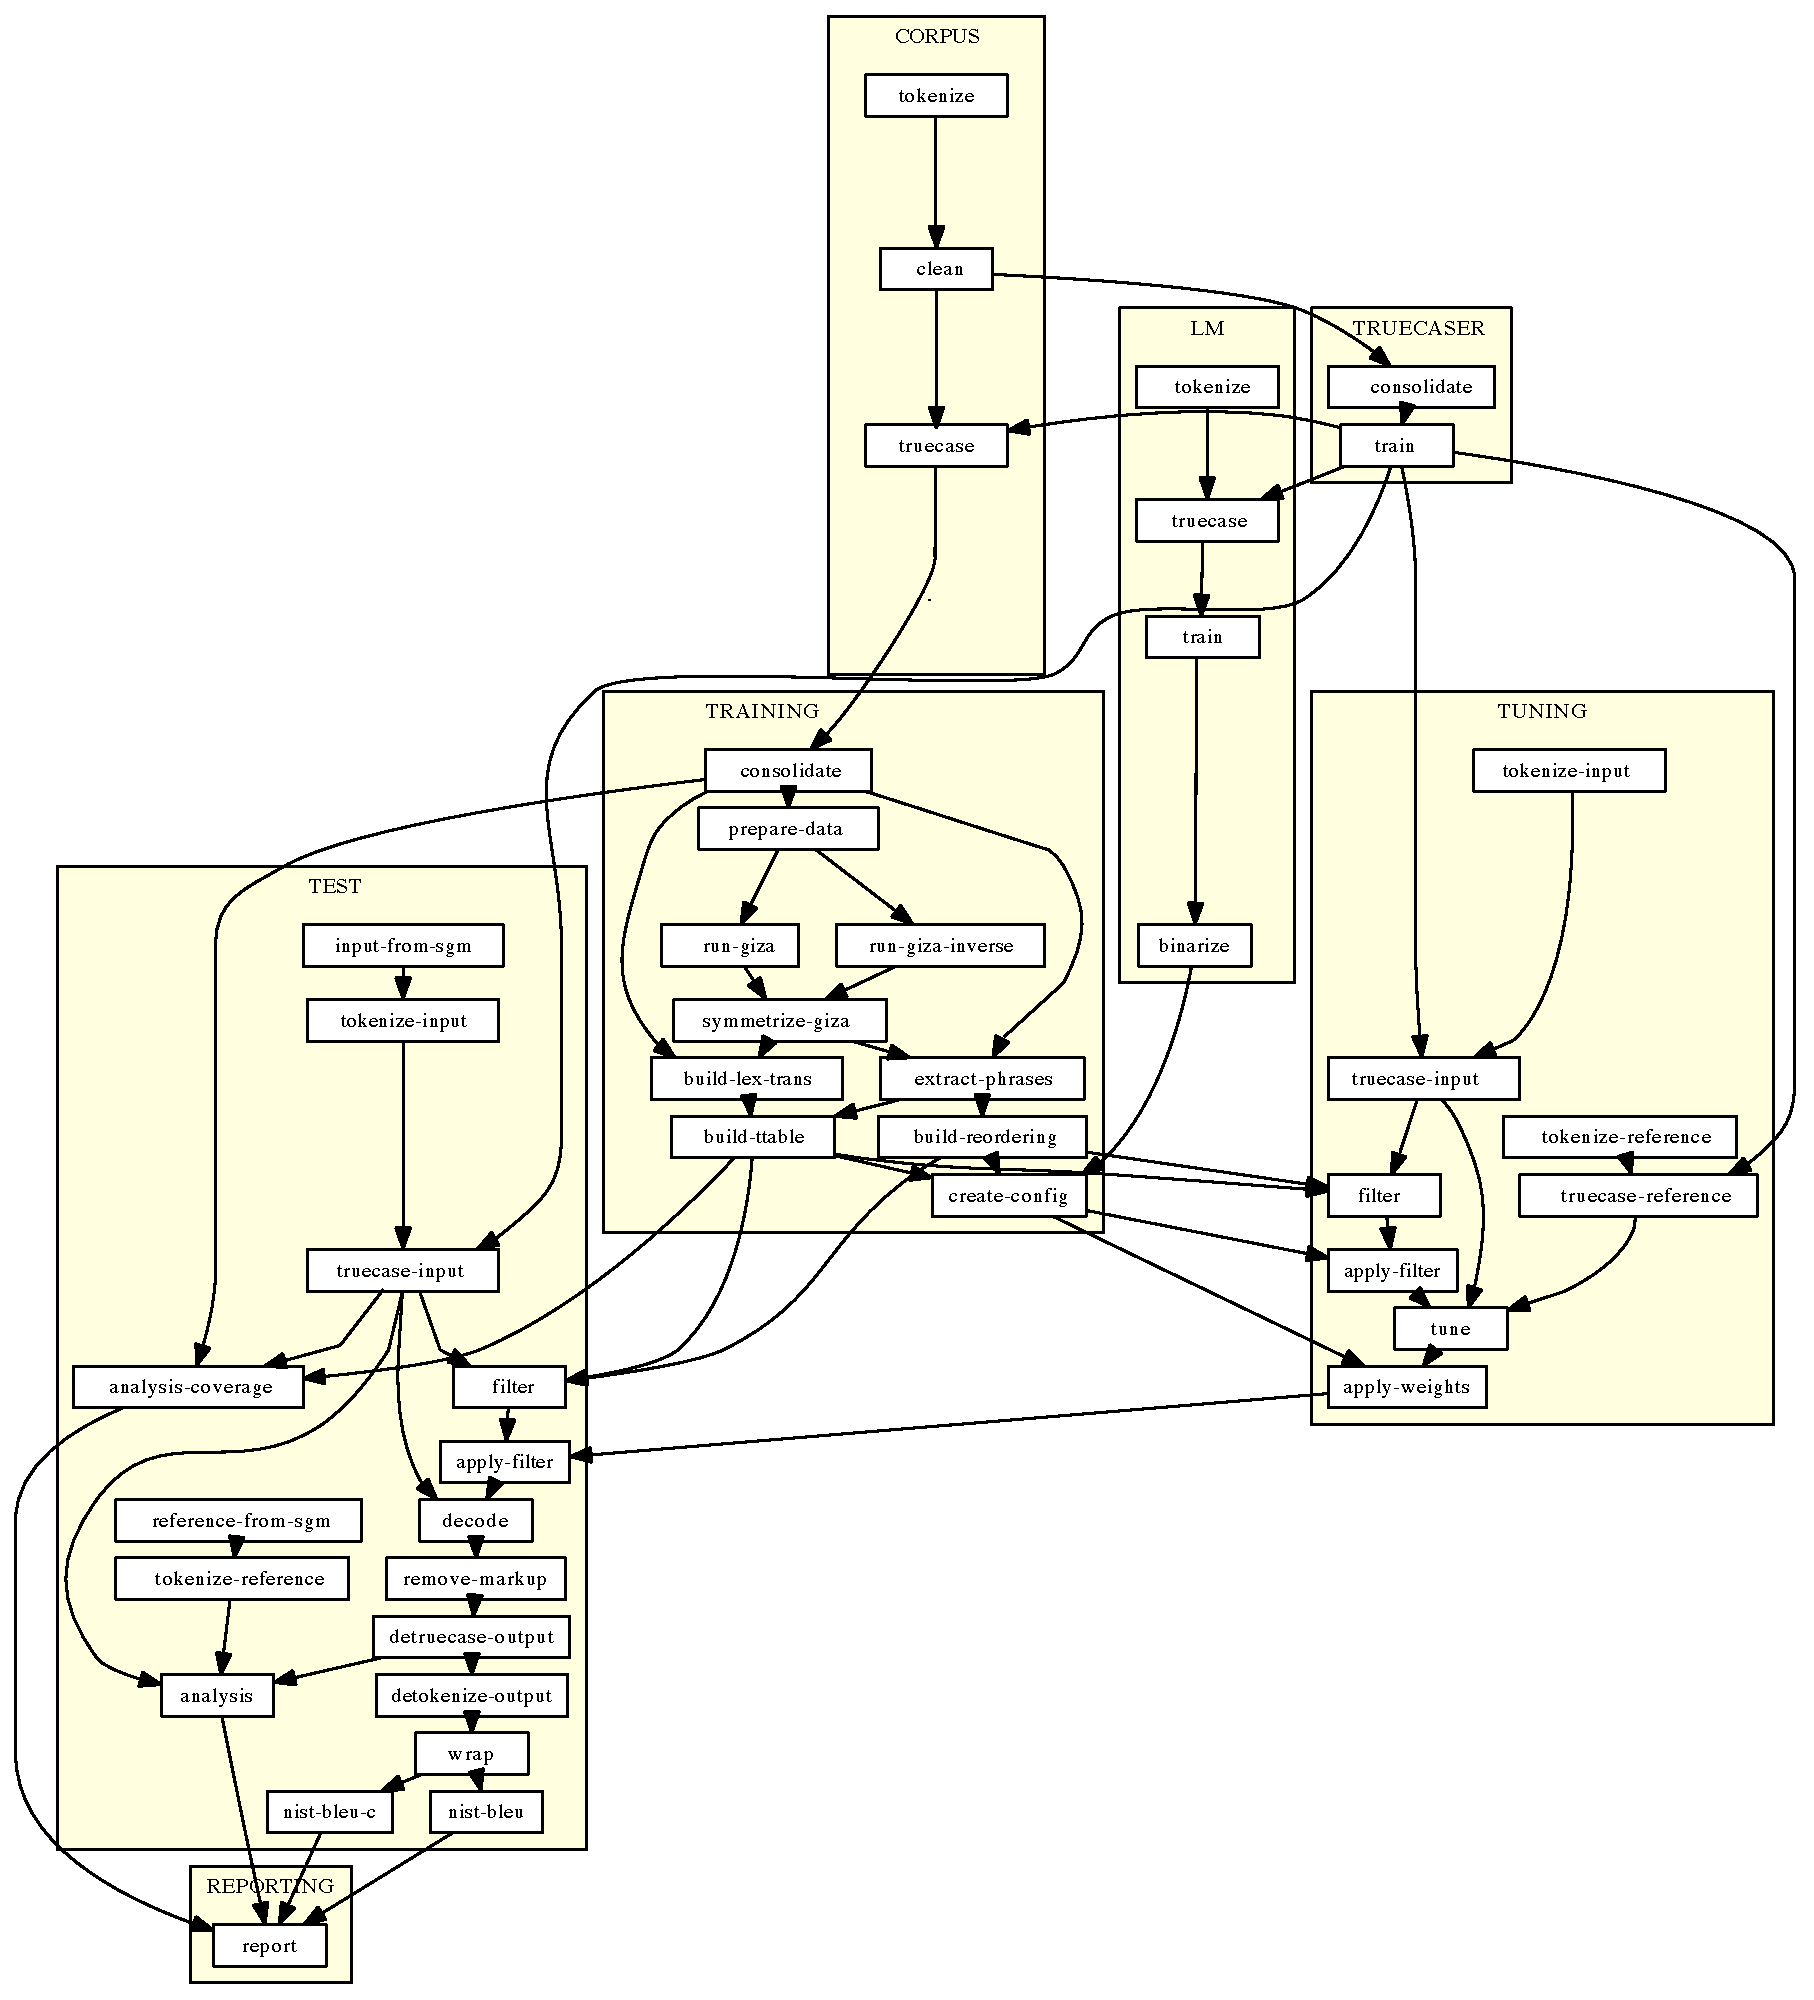
\includegraphics[width=0.8\textwidth]{figures/moses_13_graf.pdf}
\end{center}
\caption{Initial EMS set-up}\label{moses:initial}
\end{figure}

We can see the initial set-up on the Figure~\ref{moses:initial}.
\subsection{Initial results}

The initial results are below.

\begin{table}[h]
\begin{center}
\begin{tabular}{|l|l|r|}
    \hline
    \textbf{Type} & \textbf{BLEU} & \textbf{incomplete average time per sentence} \\ \hline
    Initial set-up & 23.88 & 147\,ms \\ \hline
    Google Translate & 19.07 & N/A \\  \hline
\end{tabular}
\end{center}

\caption{Initial results}\label{moses:initialresults}
\end{table}

We were very pleasantly surprised that our initial results were better than Google Translate, without really doing anything ``smart'' on our part. This is, however, definitely caused by smaller domain. On the \texttt{newstest2012} set, Google's results were still quite good, while ours were terribly low\todo{I don't have time to show concrete numbers now. If I have more time, will do.}; the phrases in newspapers are completely different than phrases in newspapers.

The time looked good on the first glance; however, real times observed didn't line up with the results with the model. The difference was actually caused by EMT filtering (seen on \ref{moses:initial} as ``filter''). EMT, before doing the final tests, actually filters the models in such a way that only needed parts are loaded; the actual time of the final test is, then, much lower.

Also, even when we didn't optimized for time, spent on initial learning, the learning phase was too long to make any experiments effective. We addressed that, too.

\section{Changes in the set-up}
\subsection{Tuning set size}
The biggest issue with the training was actually the MERT tuning. If we cut down the number of phrases for MERT tuning, the time for tuning decreases significantly, while the BLEU doesn't decrease that much.
\begin{table}[h]
\begin{center}
\begin{tabular}{|l|l|r|}
    \hline
    \textbf{Tuning size} & \textbf{BLEU} & \textbf{Tuning time} \\ \hline
    15,000 & 23.88 & 12 hours 57 minutes \\ \hline
    1,000 & 22.95 & 16 minutes \\  \hline
\end{tabular}
\end{center}

\caption{Tuning set size decrease}\label{moses:initialresults}
\end{table}

\subsection{Turning off the filtering}
To know the real time of the translation, we needed to turn off the filtering in EMT, which required some slight modification in the source code. 

However, after that, we found out, that unfiltered models simply won't fit into the memory of the machine. Therefore, we had to both binarize the models and prune the phrase table.

\subsection{Pruning the phrase table}
Finding \todo{ahem... I am tired now}stuff in the translation table takes the most time from the translation task. Therefore, making it smaller would make the translation task quicker.

As a first idea, we tried to prune the phrase table by using some factoring like short stems instead of full words. However, this showed up as a dead end; too short stems produce absolutely empty phrase table, and longer stems doesn't shrink the phrase table significantly.

Instead, we tried another method, described in one of the papers\footnote{H. Johnson, J. Martin, G. Foster and R. Kuhn. (2007) \emph{Improving Translation Quality by Discarding Most of the Phrasetable}. In Proceedings of the 2007 Joint Conference on Empirical Methods in Natural Language Processing and Computational Natural Language Learning (EMNLP-CoNLL), pp. 967-975.}. It prunes the table using statistical signifance test, called Fisher's exact test\footnote{\url{http://en.wikipedia.org/wiki/Fisher's_exact_test}}. 

This method is implemented in Moses in \texttt{sigtest-filter} script; however, EMS doesn't support it in the main Moses repo. We had to add the support for it to EMS, only to find out afterwards that Aleš Tamchyna from ÚFAL has already did that already.

As described in the original paper, pruning the table actually did increase the BLEU score; what we lost by decreasing the tuning size we got back by doing the pruning. 

\begin{table}[h]
\begin{center}
\begin{tabular}{|l|l|r|}
    \hline
    \textbf{Pruning} & \textbf{BLEU} & \textbf{ttable size (gunzipped)} \\ \hline
    No & 22.59 & 2.10 GB \\ \hline
    Yes & 23.26 & 598MB \\  \hline
\end{tabular}
\end{center}

\caption{Pruning the phrase table}\label{moses:tablepruning}
\end{table}

\subsection{Binarizing the models}
All the models - reordering model, language model and translation table (both pruned and upruned) - can be binarized. \todo{informal}What binarizing does is writing the table in such a format that can be read from disk and loaded to memory only on-demand.

Loading from disk is slower, than reading from memory, so binarizing is not helping us making the translation go quicker. However, it is helping us in fitting the models into memory at all.

\todo{table I guess}

\subsection{Smaller cube pruning}
\todo{this}todo: find out what that is actually about

I just decreased the cube pruning stack size and it just got faster.... I am not sure why. Find out!